\section{Coeficientes CAPECO}

\subsection{Coeficientes CAPECO originales - 2001}

\subsubsection{Tabla de coeficientes de Condición de Percepción utilizados para la construcción de CAPECO 2001}

\begin{figure}[h]
	\centering
	\textbf{Tabla de coeficientes de Condición de Percepción utilizados para la construcción de CAPECO}\par\medskip
	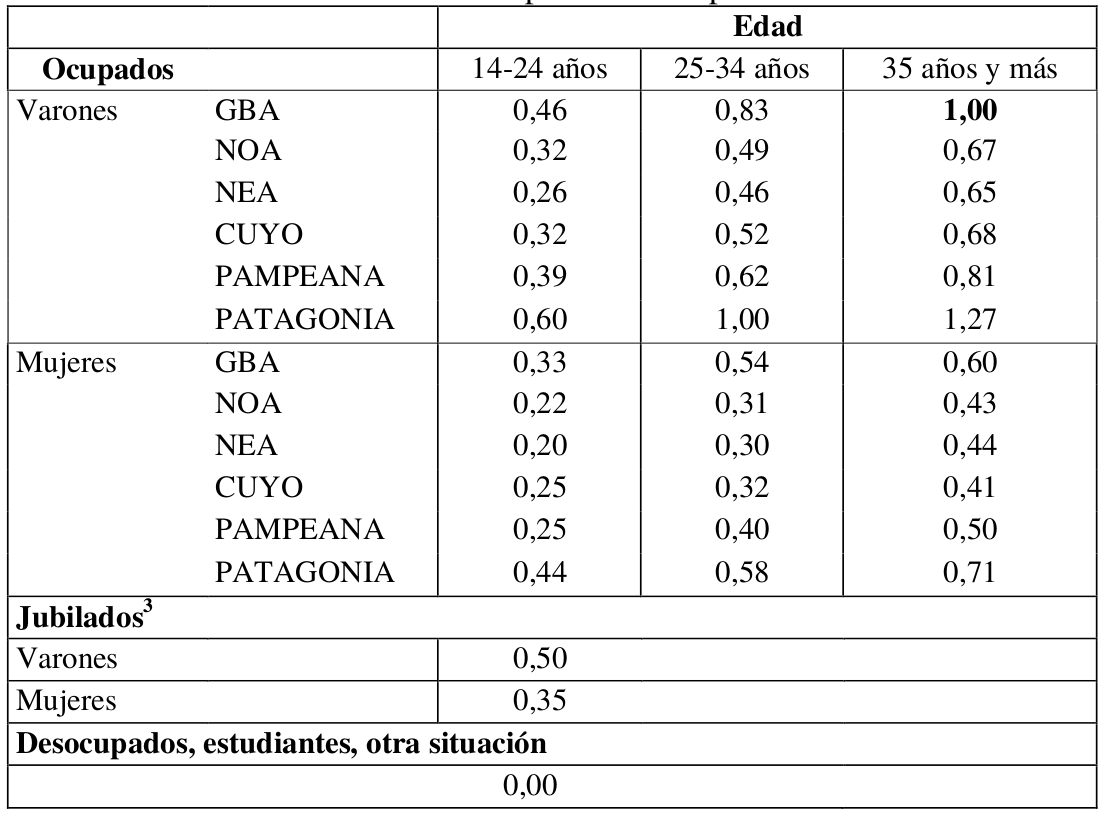
\includegraphics[scale = 0.2]{../img/anexo/capecoOriginalCP.png}
	\caption{Coeficiente de percepción del CAPECO según edad región y sexo}
\end{figure}

\subsubsection{Tabla de coeficientes de VAE utilizados para la construcción de CAPECO 2001}

\begin{table}[h!]
	\small
	\centering
	\caption{Tabla de transformación de los años de escolaridad aprobados respecto del valor en el mercado laboral del séptimo año de educación de un varón de 35 años y más de GBA}
	\label{tab:tableVAE2001}
	\begin{tabular}{p{1cm}|p{3cm}}
		Años aprobados & Valor de los años de escolaridad aprobados
		reescalados al individuo testigo \\
		\hline
		0 & 4,0\\
		\hline
		1 & 4,4\\
		\hline
		2 & 4,7\\
		\hline
		3 & 5,1\\
		\hline
		4 & 5,5\\
		\hline
		5 & 6,0\\
		\hline
		6 & 6,5\\
		\hline
		7 & 7,0\\
		\hline
		8 & 7,7\\
		\hline
		9 & 8,4\\
		\hline
		10 & 9,2\\
		\hline
		11 & 10,1\\
		\hline
		12 & 11,1\\
		\hline
		13 & 12,6\\
		\hline
		14 & 14,4\\
		\hline
		15 & 16,4\\
		\hline
		16 & 18,6\\
		\hline
		17 & 21,2\\
		
	\end{tabular}
\end{table}

\subsection{Coeficientes CAPECO actualizado - 2010}

\subsection{Adulto equivalente CAPECO original - 2001}\label{anexo}